% Transcription littérale du TD 06.
% Les abréviations et l'ordre des raisonnements de la copie sont conservés.

\exercise{53}{}

\begin{statementbox}
Lundi 12 Octobre

53| Soit $(z_n)_{n \in \N^*} \in (\C^*)^{\N^*} / \forall n \neq m \in \N^2$, $|z_n - z_m| \geq 1$. Mq $\sum \frac{1}{z_n^3}$ cv.
$\big[$Pour $R>0$, si $\#\{k \in \N^*, |z_k| \leq R\} = N(R)$, mq $N(R) \leq (2R+1)^2$.
$\cdot$ Mq on peut réordonner $(z_n)_{n \geq 1}$ de sorte que $(|z_{\tau(n)}|)_{n \geq 1}$ soit croissante (avec $\tau$ permutation de $\N$) ; conclure $\big]$
\end{statementbox}

\begin{solution}
\begin{center}
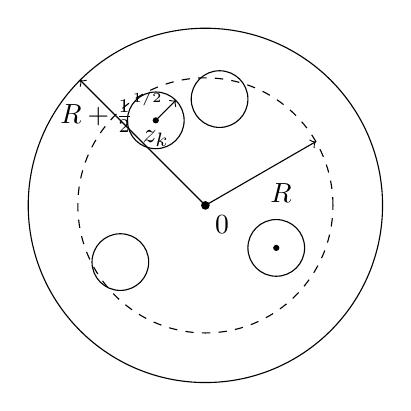
\begin{tikzpicture}[scale=0.9]
  \draw (0,0) circle (2.5cm);
  \draw[dashed] (0,0) circle (1.8cm);
  \filldraw (0,0) circle (1.5pt) node[below right] {$0$};
  \draw[->] (0,0) -- (135:2.5) node[midway, above left] {$R+\frac{1}{2}$};
  \draw[->] (0,0) -- (30:1.8) node[midway, below right] {$R$};
  
  \draw (-0.7, 1.2) circle (0.4cm);
  \filldraw (-0.7, 1.2) circle (1pt) node[below] {$z_k$};
  \draw[->] (-0.7, 1.2) -- ++(45:0.4) node[midway, above left=-2pt] {\tiny $1/2$};
  
  \draw (1.0, -0.6) circle (0.4cm);
  \filldraw (1.0, -0.6) circle (1pt);
  
  \draw (-1.2, -0.8) circle (0.4cm);
  \draw (0.2, 1.5) circle (0.4cm);
\end{tikzpicture}
\end{center}

Soit $R>0$ ; supposons que $\#\{k \in \N^*, |z_k| \leq R\} = N(R)$ (éventuellement $+\infty$).

Soient $n \neq m \in \N^2$. S'il existe $z \in \C$ tel que $|z-z_n| < \frac{1}{2}$ et $|z-z_m| < \frac{1}{2}$, alors on aurait :
\[ |z_n-z_m| < 1 \]
ce qui n'est pas. Donc les disques $\left(D\left(z_n, \frac{1}{2}\right)\right)_{n \in \N^*}$ sont 2 à 2 disjoints.
(avec $\forall z \in \C, \forall r > 0 \quad D(z,r) = \{\xi \in \C \mid |z-\xi| < r\}$)

Ces disques ont une aire de $\frac{\pi}{4}$.
De plus :
\[ \forall k \in I_R : D\left(z_k, \frac{1}{2}\right) \subset D\left(0, R+\frac{1}{2}\right) \]
car $\forall z \in D\left(z_k, \frac{1}{2}\right) : |z| \leq \underbrace{|z-z_k|}_{< 1/2} + \underbrace{|z_k|}_{\leq R} \leq R + \frac{1}{2}$.

Ainsi, en comparant les aires :
\[ \frac{\pi}{4} \times N(R) \leq \pi \left(R+\frac{1}{2}\right)^2 \]
D'où $N(R) \leq (2R+1)^2$ (et donc $N(R)$ est fini).

\begin{remarkbox}
Rem : On peut aussi observer que si $\{k \in \N^*, |z_k| \leq R\}$ était infini, on pourrait extraire une sous-suite bornée, donc (BW) une sous-suite convergente. Or si $\lim_{n \to +\infty} z_{\varphi(n)} = l \in \C$, alors :
\[ \lim_{n \to +\infty} \underbrace{|z_{\varphi(n+1)} - z_{\varphi(n)}|}_{\geq 1} = 0 \]
ce qui est impossible.
\end{remarkbox}

$\cdot$ En particulier $I_{|z_1|} = \{k \in \N^* \mid |z_k| \leq |z_1|\}$ est fini et non vide (car $1 \in I_{|z_1|}$), donc on peut définir :
\[ \tau(1) = \min \left\{ k \in I_{|z_1|} \mid |z_k| = \min_{i \in I_{|z_1|}} |z_i| \right\} \]

Soit $n \in \N^*$. Supposons $\tau(1), \dots, \tau(n)$ définis tels que $|z_{\tau(1)}| \leq \dots \leq |z_{\tau(n)}|$.
Soit $k_0 \in \N^* \setminus \{\tau(1), \dots, \tau(n)\}$. On définit :
\[ \tau(n+1) = \min \left\{ k \in I_{|z_{k_0}|} \setminus \{\tau(1)\dots\tau(n)\} \mid |z_k| = \min_{i \in I_{|z_{k_0}|} \setminus \{\tau(1)\dots\tau(n)\}} |z_i| \right\} \]
Alors $|z_{\tau(n+1)}| \geq |z_{\tau(n)}|$.

Par définition, $\tau$ est injective, et par construction, $\tau$ est surjective.
Soit $n \in \N^*$. Comme $\forall k \in \llbracket 1, n \rrbracket, \quad |z_{\tau(k)}| \leq |z_{\tau(n)}|$, en appliquant ce qui précède à $R = |z_{\tau(n)}|$ :
\[ n \leq (2|z_{\tau(n)}|+1)^2 \]
Donc $\sqrt{n} \leq 2|z_{\tau(n)}| + 1$ et $|z_{\tau(n)}| \geq \frac{\sqrt{n}-1}{2}$.

Pour $n \geq 2$ :
\[ \frac{1}{|z_{\tau(n)}|^3} \leq \left( \frac{2}{\sqrt{n}-1} \right)^3 = \mathcal{O}\left(\frac{1}{n^{3/2}}\right) \]
C'est le terme général d'une SATP convergente (Critère de Riemann).

Ainsi $\sum_{n \geq 1} \frac{1}{z_{\tau(n)}^3}$ converge absolument. Donc $\left( \frac{1}{z_{\tau(n)}^3} \right)_{n \in \N^*}$ est sommable, ce qui implique que $\left( \frac{1}{z_n^3} \right)_{n \in \N^*}$ est aussi sommable.

\begin{remarkbox}
Rem : On peut avoir $\sum \frac{1}{|z_n|^2}$ divergente.
\end{remarkbox}
\end{solution}

\exercise{75}{}

\begin{statementbox}
75| 
a) Nature des séries $\sum_{n \ge 1} \frac{\ln n}{n}$ et $\sum_{n \ge 1} (-1)^n \frac{\ln n}{n}$ \\
b) Soit pour $N \in \N^*, S_N = \sum_{n=1}^N \frac{\ln n}{n}$ ; mq $\left(S_N - \frac{\ln^2(N)}{2}\right)_{N \ge 1}$ (cv). \\
c) On forme $\forall N \ge 1, \quad T_N = \sum_{n=1}^N \frac{(-1)^n \ln n}{n}$ ; en évaluant $T_{2N}$, calculer $\sum_{n=1}^{+\infty} \frac{(-1)^n \ln n}{n}$.
\end{statementbox}

\begin{solution}
\partanswer{a)}
On a $\frac{1}{n} \underset{n \to +\infty}{=} o\left(\frac{\ln n}{n}\right)$, donc la SATP $\sum_{n \geq 1} \frac{\ln n}{n}$ \boxed{\text{dv}}.

Soit $f : [1; +\infty[ \to \R \quad \mathcal{C}^1$, telle que $t \mapsto \frac{\ln t}{t}$. 
\[ \forall t \geq 1, \quad f'(t) = \frac{1-\ln t}{t^2} \]
Et $\forall t \geq e, \quad f'(t) \leq 0$, donc $f$ est décroissante sur $[e; +\infty[$.
La suite $\left( \frac{\ln n}{n} \right)_{n \geq 3}$ est donc décroissante.
Comme $\lim_{n \to +\infty} \frac{\ln n}{n} = 0$, d'après le C.S.S.A., $\sum (-1)^n \frac{\ln n}{n}$ \boxed{\text{cv}}.

\partanswer{b)}
Soit $x_N = S_N - \frac{\ln^2 N}{2}$. Pour $N \geq 2$ :
\[ x_N - x_{N-1} = \frac{\ln N}{N} - \frac{\ln^2(N)}{2} + \frac{\ln^2(N-1)}{2} \]
Or :
\begin{align*}
\ln(N-1) &= \ln\left(N\left(1-\frac{1}{N}\right)\right) = \ln N + \ln\left(1-\frac{1}{N}\right) \\
&= \ln N - \frac{1}{N} + \mathcal{O}\left(\frac{1}{N^2}\right)
\end{align*}
D'où :
\[ \ln^2(N-1) = \ln^2(N) - 2\frac{\ln(N)}{N} + \mathcal{O}\left(\frac{\ln N}{N^2}\right) \]
Donc :
\[ x_N - x_{N-1} = \mathcal{O}\left(\frac{\ln N}{N^2}\right) = \mathcal{O}\left(\frac{1}{N^{3/2}}\right) \]
qui est le terme général d'une série absolument convergente.

La série $\sum (x_N - x_{N-1})$ \boxed{\text{cv}}, donc la suite $\left(x_N = S_N - \frac{\ln^2(N)}{2}\right)_{N \geq 1}$ \boxed{\text{cv}}.
Et $\exists C \in \R$ tel que $S_N = \frac{\ln^2(N)}{2} + C + o(1)$.

\partanswer{c)}
\begin{align*}
T_{2N} &= \sum_{n=1}^{2N} (-1)^n \frac{\ln n}{n} \\
&= \sum_{p=1}^N \frac{\ln(2p)}{2p} - \sum_{p=0}^{N-1} \frac{\ln(2p+1)}{2p+1} \\
&= \frac{\ln 2}{2} H_N + \frac{1}{2} S_N - \sum_{p=0}^{N-1} \frac{\ln(2p+1)}{2p+1}
\end{align*}
De même :
\[ S_{2N} = \frac{\ln 2}{2} H_N + \frac{1}{2} S_N + \sum_{p=0}^{N-1} \frac{\ln(2p+1)}{2p+1} \]

En additionnant, il vient : 
\[ T_{2N} + S_{2N} = \ln 2 \times H_N + S_N \]
Soit :
\[ T_{2N} = \ln 2 \times H_N + S_N - S_{2N} \]
Or $H_N = \ln N + \gamma + o(1)$. Calculons $S_N - S_{2N}$ :
\begin{align*}
S_N - S_{2N} &= \frac{(\ln N)^2}{2} - \frac{(\ln 2N)^2}{2} + o(1) \\
&= \frac{(\ln N)^2}{2} - \frac{1}{2} \left[ (\ln 2)^2 + 2\ln 2 \ln N + (\ln N)^2 \right] + o(1) \\
&= -\ln 2 \ln N - \frac{(\ln 2)^2}{2} + o(1)
\end{align*}
Ainsi :
\begin{align*}
T_{2N} &= \ln 2 \times (\ln N + \gamma) - \ln 2 \ln N - \frac{(\ln 2)^2}{2} + o(1) \\
&= \gamma \ln 2 \cancel{+\ln 2 \ln N} \cancel{- \ln 2 \ln N} - \frac{(\ln 2)^2}{2} + o(1)
\end{align*}
Il s'en suit, lorsque $N \to +\infty$ que :
\[ \boxed{\sum_{n=1}^{+\infty} (-1)^n \frac{\ln n}{n} = \gamma \ln 2 - \frac{(\ln 2)^2}{2}} \]
\end{solution}

\exercise{105}{}

\begin{statementbox}
105| Soit $\sum a_n$ une série complexe abs cv.
On pose $\forall(p,q) \in (\N^*)^2 \quad u_{p,q} = \begin{cases} 0 & \text{si } p > q \\ \frac{p a_p}{q(q+1)} & \text{si } p \leq q \end{cases}$
Mq $(u_{p,q})_{(p,q)\in(\N^*)^2}$ est sommable, et calculer sa somme en fonction de $\sum a_n$.
\end{statementbox}

\begin{solution}
Dans $\R \cup \{+\infty\}$, soit $p \in \N^*$ fixé :
\begin{align*}
\sum_{q=1}^{+\infty} |u_{p,q}| &= \sum_{q=p}^{+\infty} \frac{p |a_p|}{q(q+1)} \\
&= p |a_p| \sum_{q=p}^{+\infty} \frac{1}{q(q+1)} \\
&= p |a_p| \sum_{q=p}^{+\infty} \left( \frac{1}{q} - \frac{1}{q+1} \right) \\
&= p |a_p| \frac{1}{p} = |a_p| \quad \text{(série télescopique)}
\end{align*}

Ainsi :
\[ \sum_{p=1}^{+\infty} \left( \sum_{q=1}^{+\infty} |u_{p,q}| \right) = \sum_{p=1}^{+\infty} |a_p| < +\infty \]
Donc $(u_{p,q})_{(p,q)\in(\N^*)^2}$ est sommable (d'après le Thm de SPP pour des réels $\geq 0$).

D'après le Thm de S.P.P. :
\[ \sum_{(p,q)\in(\N^*)^2} u_{p,q} = \sum_{p=1}^{+\infty} \sum_{q=1}^{+\infty} u_{p,q} = \sum_{p=1}^{+\infty} a_p \]

Ceci montre que $\sum_{q \geq 1} v_q$ converge (avec $\forall q \geq 1, \quad v_q = \sum_{p=1}^q u_{p,q} = \frac{1}{q(q+1)} \sum_{p=1}^q p a_p$).
\[ \sum_{q=1}^{+\infty} v_q = \sum_{p=1}^{+\infty} a_p \]

\begin{remarkbox}
Rem : Si les $a_p \geq 0$, ce résultat reste valable en cas de dv ; par ex. si $a_p = \frac{1}{p} \quad \forall p \geq 1$.
Si $a_p = \frac{1}{p^2}$ :
\[ v_q = \frac{1}{q(q+1)} \sum_{p=1}^q \frac{1}{p} \sim \frac{\ln q}{q^2} = \mathcal{O}\left(\frac{1}{q^{3/2}}\right) \]
et $\sum_{q=1}^{+\infty} \frac{H_q}{q(q+1)} = \zeta(2) = \frac{\pi^2}{6}$.
\end{remarkbox}
\end{solution}

\begin{remarkbox}
\textbf{Remarque isolée (Lien avec l'inégalité de Carleman)}

Soit $\sum u_n$ une SATP cv. Soit $v_n = \sqrt[n]{u_1 \dots u_n}$.
On admet l'inégalité arithmético-géométrique (provient de la concavité du $\ln$), i.e. $\forall (a_1, \dots, a_n) \in \R_+^* : \sqrt[n]{a_1 \dots a_n} \leq \frac{a_1 + \dots + a_n}{n}$.

Il vient :
\[ \sqrt[n]{ \left(\frac{1 \cdot u_1}{n+1}\right) \left(\frac{2 \cdot u_2}{n+1}\right) \dots \left(\frac{n \cdot u_n}{n+1}\right) } \leq \frac{1}{n} \left( \frac{u_1 + 2u_2 + \dots + n u_n}{n+1} \right) \]
\[ v_n \times \frac{\sqrt[n]{n!}}{n+1} \leq \frac{1}{n(n+1)} (u_1 + 2u_2 + \dots + n u_n) \]
Le terme de droite est le terme général d'une SATP cv d'après l'exercice précédent.

\textbf{Lemme :} $\forall n \geq 1 \quad \frac{\sqrt[n]{n!}}{n+1} \geq \frac{1}{e}$ (par récurrence).

Donc :
\[ \frac{1}{e} v_n \leq v_n \frac{\sqrt[n]{n!}}{n+1} \leq \frac{1}{n(n+1)}(u_1 + 2u_2 + \dots + n u_n) \]
Ainsi, $\sum v_n$ cv et $\sum_{n=1}^\infty v_n \leq e \sum_{n=1}^\infty u_n$.
\end{remarkbox}

\exercise{81}{}

\begin{statementbox}
81| (Inégalité de Carleman): Soit $\sum u_n$ SATP cv.
a) On pose $v_n = \frac{1}{n(n+1)} \sum_{p=1}^n p u_p$. Mq $\sum v_n$ cv et $\sum_{n=1}^{+\infty} v_n = \sum_{n=1}^{+\infty} u_n$. \\
b) On admet l'inégalité arithmético-géométrique: $\forall (a_1 \dots a_n) \in \R_+^* \quad \sqrt[n]{a_1 \dots a_n} \leq \frac{a_1 + \dots + a_n}{n}$. Justifier que $\frac{\sqrt[n]{n!}}{n+1} \times \sqrt[n]{u_1 \dots u_n} \leq v_n$. \\
c) En déduire que $\sum \sqrt[n]{u_1 \dots u_n}$ cv et que $\sum_{n=1}^{+\infty} \sqrt[n]{u_1 \dots u_n} \leq e \sum_{n=1}^{+\infty} u_n$. \\
d) Montrer que $e$ est la meilleure constante possible.
\end{statementbox}

\begin{solution}
\partanswer{a)}
Soit pour $(n,p) \in (\N^*)^2 \quad \alpha_{n,p} = \begin{cases} \frac{p u_p}{n(n+1)} & \text{si } p \leq n \\ 0 & \text{sinon} \end{cases}$.

Dans $\R \cup \{+\infty\}$, d'après le Théorème de Fubini pour des réels $\geq 0$ :
\begin{align*}
\sum \alpha_{n,p} &= \sum_{n=1}^{+\infty} \sum_{p=1}^{+\infty} \alpha_{n,p} = \sum_{n=1}^{+\infty} \sum_{p=1}^n \alpha_{n,p} = \sum_{n=1}^{+\infty} v_n \\
&= \sum_{p=1}^{+\infty} \sum_{n=p}^{+\infty} \alpha_{n,p} = \sum_{p=1}^{+\infty} \sum_{n=p}^{+\infty} \frac{p u_p}{n(n+1)} \\
&= \sum_{p=1}^{+\infty} p u_p \underbrace{\left( \sum_{n=p}^{+\infty} \frac{1}{n(n+1)} \right)}_{= \frac{1}{p} \text{ (télescopique)}} \\
&= \sum_{p=1}^{+\infty} u_p < +\infty
\end{align*}
Donc $\sum v_n < +\infty$ et $\sum_{n=1}^{+\infty} v_n = \sum_{n=1}^{+\infty} u_n$.

\partanswer{b)}
Soit $n \geq 1$ : 
\[ \frac{\sqrt[n]{n!}}{n+1} \sqrt[n]{u_1 \dots u_n} = \sqrt[n]{\frac{u_1 \cdot 2u_2 \dots n u_n}{(n+1)^n}} \leq \frac{1}{n} \sum_{p=1}^n \frac{p u_p}{n+1} = v_n \]

\textbf{Lemme :} $\forall n \geq 1, \quad \frac{(n+1)^n}{n!} \leq e^n$.
\textbf{Dém :} Par récurrence.
Pour $n=1$ : $2 \leq e$.
Soit $n \in \N^*$, supposons $\frac{(n+1)^n}{n!} \leq e^n$. Alors :
\begin{align*}
\frac{(n+2)^{n+1}}{(n+1)!} &= \frac{(n+1)^n}{n!} \times \frac{(n+2)^{n+1}}{(n+1)^{n+1}} \times \frac{1}{n+1} \\
&\leq e^n \left( 1 + \frac{1}{n+1} \right)^{n+1}
\end{align*}
Or :
\[ \left(1+\frac{1}{n+1}\right)^{n+1} = \exp\left((n+1)\ln\left(1+\frac{1}{n+1}\right)\right) \leq e \]
D'où $\frac{(n+2)^{n+1}}{(n+1)!} \leq e^{n+1}$.

\partanswer{c)}
Comme $n \geq 1$, on a $\sqrt[n]{u_1 \dots u_n} \leq \frac{n+1}{\sqrt[n]{n!}} v_n \leq e \cdot v_n$ d'après le lemme.
Donc $\sum \sqrt[n]{u_1 \dots u_n} < +\infty$ et :
\[ \sum_{n=1}^{+\infty} \sqrt[n]{u_1 \dots u_n} \leq e \sum_{n=1}^{+\infty} v_n = e \sum_{n=1}^{+\infty} u_n \]

\partanswer{d)}
Soit $C > 0$ tel que pour toute $\sum u_n$ SATP cv, on ait $\sum_{n=1}^{+\infty} \sqrt[n]{u_1 \dots u_n} \leq C \sum_{n=1}^{+\infty} u_n$.

Soit $N > 0$ et $u_n^{(N)} = \begin{cases} \frac{1}{n!} & \text{si } n \leq N \\ 0 & \text{si } n > N \end{cases}$.
La somme donne $\sum_{n=1}^{+\infty} u_n^{(N)} = \sum_{n=1}^N \frac{1}{n!}$.
Ainsi, $\forall N \geq 1$,
\[ \sum_{n=1}^N \frac{1}{\sqrt[n]{n!}} \leq C H_N \]

Où $\forall n \geq 1$, 
\begin{align*}
\sqrt[n]{n!} &= \exp\left(\frac{1}{n}\ln(n!)\right) \\
&= \exp\left(\frac{1}{n}\ln\left(n^n e^{-n} \sqrt{2\pi n} (1+o(1))\right)\right) \\
&= \exp\left( \ln(n) - 1 + o(1) \right) \sim \frac{n}{e}
\end{align*}
Donc $\frac{1}{\sqrt[n]{n!}} \sim_{n \to \infty} \frac{e}{n}$ qui est le terme général d'une SATP dv.

D'après le théorème de sommation des relations de comparaison :
\[ \sum_{n=1}^N \frac{1}{\sqrt[n]{n!}} \sim e H_N \]
Alors $\frac{\sum_{n=1}^N \frac{1}{\sqrt[n]{n!}}}{H_N} \leq C$.
Pour $N \to +\infty$, on obtient $\boxed{e \leq C}$.
\end{solution}

\exercise{108}{}

\begin{statementbox}
108| Soit pour $n \in \N^*, d(n)$ le nb de diviseur de $n$. Mq $\sum_{n=1}^\infty d(n)e^{-n} = \sum_{p=1}^\infty \frac{e^{-p}}{1-e^{-p}}$.
\end{statementbox}

\begin{solution}
Soit $p \geq 1$. On a $0 < e^{-p} < 1$, donc :
\[ \frac{e^{-p}}{1-e^{-p}} = e^{-p} \sum_{n=0}^{+\infty} (e^{-p})^n = \sum_{n=0}^{+\infty} e^{-p(n+1)} = \sum_{n=1}^{+\infty} e^{-pn} \]
On remarque que $0 < \frac{e^{-p}}{1-e^{-p}} \sim_{p \to +\infty} e^{-p}$, qui est le terme général d'une série géométrique convergente.

Dans $\R_+$ :
\[ \sum_{p=1}^{+\infty} \frac{e^{-p}}{1-e^{-p}} = \sum_{p=1}^{+\infty} \sum_{n=1}^{+\infty} e^{-pn} = \sum_{(n,p)\in(\N^*)^2} e^{-np} < +\infty \]
Soit pour $k \in \N^*, \quad I_k = \{(n,p) \in (\N^*)^2 \mid np = k\}$.
On a $(\N^*)^2 = \bigcup_{k \in \N^*} I_k$.

Par le Théorème de Fubini (SPP pour $\R_+$) :
\[ \sum_{p=1}^{+\infty} \frac{e^{-p}}{1-e^{-p}} = \sum_{k=1}^{+\infty} \sum_{(n,p) \in I_k} e^{-k} = \sum_{k=1}^{+\infty} (\# I_k) e^{-k} = \sum_{k=1}^{+\infty} d(k) e^{-k} \]
\end{solution}

\exercise{86}{}

\begin{statementbox}
86| Soit pour $n \in \N^*, d(n)$ le nombre de diviseurs de $n$.
Mq. $\forall z \in \C, |z|<1$, on a $\sum_{n=1}^{+\infty} d(n)z^n = \sum_{k=1}^{+\infty} \frac{z^k}{1-z^k}$.
\end{statementbox}

\begin{solution}
Soit $k \geq 1$, on a $|z^k| < 1$ donc :
\[ \frac{1}{1-z^k} = \sum_{p=0}^{+\infty} z^{pk} \]

Raisonnons dans $\R_+ \cup \{+\infty\}$, d'après le théorème de SPP pour des réels $\geq 0$ :
\[ \sum_{k=1}^{+\infty} \sum_{p=0}^{+\infty} |z|^{k(1+p)} = \sum_{k=1}^{+\infty} \frac{|z|^k}{1-|z|^k} \]
Or $\frac{|z|^k}{1-|z|^k} \sim |z|^k$, qui est le terme général d'une série géométrique convergente.
Donc la famille $(z^{k(1+p)})_{(k,p)\in \N^* \times \N}$ est sommable.

D'après le théorème de sommation par paquets (SPP) :
\[ \sum_{k=1}^{+\infty} \frac{z^k}{1-z^k} = \sum_{(k,p)\in \N^* \times \N} z^{k(p+1)} = \sum_{(k,p)\in (\N^*)^2} z^{kp} \]

En posant $I_n = \{(k,p) \in (\N^*)^2 \mid kp = n\}$, on a $\bigcup_{n \in \N^*} I_n = (\N^*)^2$.
\[ \sum_{k=1}^{+\infty} \frac{z^k}{1-z^k} = \sum_{n=1}^{+\infty} \sum_{(k,p) \in I_n} z^n = \sum_{n=1}^{+\infty} |I_n| z^n \]
L'application $D(n) \to I_n, \quad d \mapsto \left(d, \frac{n}{d}\right)$ est une bijection, d'où $|I_n| = d(n)$.
Donc :
\[ \sum_{k=1}^{+\infty} \frac{z^k}{1-z^k} = \sum_{n=1}^{+\infty} d(n)z^n \]

\begin{remarkbox}
Rem : Si $n = \prod_{p \in \mathcal{P}} p^{v_p(n)}$ (produit fini : $\{p \in \mathcal{P} \mid v_p(n) \geq 1\}$ est fini), on a :
\[ d(n) = \prod_{p \in \mathcal{P}} (v_p(n) + 1) \]
On peut mq $\forall \varepsilon > 0, \quad d(n) = \mathcal{O}(n^\varepsilon)$
ssi $\exists M > 0 \text{ t.q. } \forall n \geq 1, \quad d(n) \leq M n^\varepsilon$
ssi $\exists M > 0 \text{ t.q. } \forall n \geq 1, \quad \ln(d(n)) \leq \ln M + \varepsilon \ln n$
\[ \sum_{p \in \mathcal{P}} \ln(v_p(n)+1) \leq \ln M + \varepsilon \sum_{p \in \mathcal{P}} v_p(n) \ln p \]
Il faut vérifier que $\sum_{p \in \mathcal{P}} (\ln(v_p(n)+1) - \varepsilon v_p(n) \ln p)$ est majorée indépendamment des $(v_p(n))_{p \in \mathcal{P}} \dots$
\end{remarkbox}
\end{solution}

\exercise{106}{}

\begin{statementbox}
106| Soit $\alpha \in \R$.
a) Donner une CNS sur $\alpha$ pour que $\left(\frac{1}{(p+q)^\alpha}\right)_{(p,q)\in \N^2 \setminus \{(0,0)\}}$ soit sommable, exprimer alors la somme en fonction de $\zeta$. \\
b) même question pour $\left(\frac{1}{(p^2+q^2)^\alpha}\right)_{(p,q)\in \N^2 \setminus \{(0,0)\}}$ (on vérifiera que $\frac{1}{2}(p+q)^2 \leq p^2+q^2 \leq (p+q)^2$).
\end{statementbox}

\begin{solution}
\partanswer{a)}
D'après le Thm de SPP pour des réels $\geq 0$.
Soit pour $n \in \N^*, \quad I_n = \{(p,q) \in \N^2 \mid p+q=n\}$.
On a $\N^2 \setminus \{(0,0)\} = \bigcup_{n \in \N^*} I_n$.
\begin{align*}
\sum_{(p,q)\in \N^2 \setminus \{(0,0)\}} \frac{1}{(p+q)^\alpha} &= \sum_{n \in \N^*} \sum_{(p,q) \in I_n} \frac{1}{n^\alpha} \\
&= \sum_{n \in \N^*} |I_n| \frac{1}{n^\alpha} \\
&= \sum_{n \in \N^*} \frac{n+1}{n^\alpha} \sim \frac{1}{n^{\alpha-1}}
\end{align*}
Il y a CV ssi $\alpha - 1 > 1 \iff \boxed{\alpha > 2}$.

Pour $\alpha > 2$ : 
\[ \sum_{(p,q) \in \N^2 \setminus \{(0,0)\}} \frac{1}{(p+q)^\alpha} = \zeta(\alpha-1) + \zeta(\alpha) \]

\partanswer{b)}
On a le lemme : $\frac{1}{2}(p+q)^2 \leq p^2+q^2 \leq (p+q)^2$.
(À gauche : $(p+q)^2 - 2(p^2+q^2) = -(p-q)^2 \leq 0$, d'où $\frac{1}{2}(p+q)^2 \leq p^2+q^2$).

Si $\alpha \leq 0$ : 
$\frac{1}{(p^2+q^2)^\alpha} \geq 1$. La famille n'est pas sommable.

Si $\alpha > 0$ : 
$\forall (p,q) \in \N^2 \setminus \{(0,0)\}$,
\[ \frac{1}{(p+q)^{2\alpha}} \leq \frac{1}{(p^2+q^2)^\alpha} \leq \frac{2^\alpha}{(p+q)^{2\alpha}} \]
D'après le a), $\left(\frac{1}{(p+q)^{2\alpha}}\right)_{(p,q)}$ est sommable ssi $2\alpha > 2 \iff \boxed{\alpha > 1}$.
Donc $\left(\frac{1}{(p^2+q^2)^\alpha}\right)$ est sommable ssi $\alpha > 1$.

\begin{remarkbox}
Rem : Définissons pour $n \in \N^* : J_n = \{(p,q) \in \N^2 \mid p^2+q^2=n\}$.
$|J_1|=2 ; |J_2|=1 ; |J_3|=0 ; |J_4|=2 ; |J_5|=2 ; |J_6|=0 ; |J_7|=0 ; |J_8|=1$.
On a :
\[ \sum_{(p,q)\in \N^2 \setminus \{(0,0)\}} \frac{1}{(p^2+q^2)^\alpha} = \sum_{n=1}^{+\infty} \frac{|J_n|}{n^\alpha} \quad \text{CV ssi } \alpha > 1 \]
On vérifiera que (Fermat) $J_n \neq \emptyset \text{ ssi } \forall p \text{ premier } \equiv 3 [4] : v_p(n) \text{ est pair}$.
\end{remarkbox}
\end{solution}

\exercise{89}{}

\begin{statementbox}
89| Soit $\sum a_n$ une série semi convergente.
a) Soit pour $n \geq 0 : a_n^+ = \max\{a_n, 0\}$ et $a_n^- = \max\{-a_n, 0\}$. Mq $\sum a_n^+$ et $\sum a_n^-$ DV. \\
b) On forme $I^+ = \{n \in \N \mid a_n \geq 0\}$ et $I^- = \{n \in \N \mid a_n < 0\}$. Soit $l \in \R$ mq $\exists \sigma : \N \to \N$ bijective / $\sum_{n=0}^{+\infty} a_{\sigma(n)} = l$.
\end{statementbox}

\begin{solution}
\partanswer{a)}
On a $a_n^+ \geq 0 ; a_n^- \geq 0$.
De plus, $a_n^+ + a_n^- = |a_n|$ et $a_n^+ - a_n^- = a_n$.

Si $\sum a_n^+$ et $\sum a_n^-$ convergeaient toutes les deux, alors $\sum |a_n|$ convergerait (absolument), ce qui n'est pas le cas.
Si l'une convergeait et l'autre divergeait, alors $\sum a_n$ divergerait, ce qui n'est pas non plus.
Donc $\sum a_n^+$ et $\sum a_n^-$ sont divergentes.

\partanswer{b)}
Soit $l \in \R_+$, et $\forall n \in \N, \quad S_n^+ = \sum_{k=0}^n a_k^+ \to +\infty$ et $S_n^- = \sum_{k=0}^n a_k^- \to +\infty$.
Notons $n_0 = \min\{n \in \N \mid S_n^+ \geq l\}$ et $n_1 = \min\{n \in \N \mid S_{n_0}^+ - S_n^- \leq l\}$.

\begin{center}
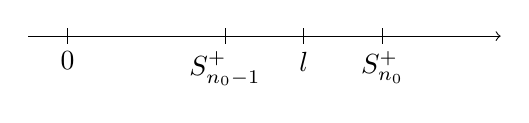
\begin{tikzpicture}
  \draw[->] (0,0) -- (6,0);
  \draw (0.5, -0.1) -- (0.5, 0.1) node[below=5pt] {$0$};
  \draw (2.5, -0.1) -- (2.5, 0.1) node[below=5pt] {$S_{n_0-1}^+$};
  \draw (3.5, -0.1) -- (3.5, 0.1) node[below=5pt] {$l$};
  \draw (4.5, -0.1) -- (4.5, 0.1) node[below=5pt] {$S_{n_0}^+$};
\end{tikzpicture}
\end{center}

Comme $\sum a_n^+$ diverge, on peut supposer :
\[ n_2 = \min\left\{n > n_0 \mid S_{n_0}^+ - S_{n_1}^- + \sum_{k=n_0+1}^n a_k^+ \geq l\right\} \]
et ainsi de suite.
On a ainsi formé une partition de $\N$.

Par définition :
\begin{align*}
0 &\leq S_{n_0}^+ - l \leq S_{n_0}^+ - S_{n_0-1}^+ = a_{n_0}^+ \\
0 &\leq l - (S_{n_0}^+ - S_{n_1}^-) \leq S_{n_1}^- - S_{n_1-1}^- = a_{n_1}^-
\end{align*}

Comme $\sum a_n$ converge, on a $a_n \to 0$ et $n_2 > n_0$, $n_3 > n_1$, \dots
Les sommes partielles obtenues convergent vers $l$.

Si $l < 0$, on procède de même avec $\sum -a_n$.

\begin{remarkbox}
Rem : Comme $\lim a_n = 0, \quad \exists \sigma : \N \to \N \text{ bijective telle que } (|a_{\sigma(n)}|)_{n \in \N} \text{ soit décroissante}$.
Car soit $m = \sup\{n \in \N \mid |a_n| > 0\}$ existe sinon $\sum |a_n|$ cv.
Et on prend $\sigma(0) \in \N$ tel que $|a_{\sigma(0)}| = \max_{k \in \N} |a_k|$.
Puis pour $\sigma(0), \dots, \sigma(n)$ construits, on prend $\sigma(n+1) \in \N$ tel que :
\[ |a_{\sigma(n+1)}| = \max_{k \in \N \setminus \{\sigma(0), \dots, \sigma(n)\}} |a_k| \]
On peut permuter les $(a_{\sigma(n)})_{n \in \N}$ pour avoir $\sum_{n=0}^{+\infty} a_{\sigma(n)} = +\infty$.
\end{remarkbox}
\end{solution}
